% !TEX root =  ICRA2012-Patil.tex

%Motion planning for robots is often complicated by real-world uncertainties; the motion of the robot may deviate unpredictably from the assumed dynamics model, and sensors might yield noisy and partial state measurements of the robot state.
%Maintaining the safety of robot motions is complicated by real-world uncertainties; the motion of the robot may deviate unpredictably from the assumed dynamics model, and sensors might yield imperfect information about the robot state due to noisy and partial state measurements.

%When computing a motion plan for a robot to execute to accomplish a task, explicitly considering uncertainty in robot motion and sensing enables computation of safer plans.
%Explicitly considering uncertainty in robot motion and sensing during motion planning enables the computation of safer plans.
%Computing safe robot motions requires a motion planner that explicitly considers uncertainty in robot motion and sensing.
For many applications ranging from autonomous vehicles to steerable medical needles operating in the human body \cite{Cowan2011_Chapter}, the motion plan chosen for execution should be as safe as possible such that there is minimal risk that the robot will collide with obstacles in the environment. Real-world uncertainties arise because the motion of the robot may deviate unpredictably from the assumed dynamics model and because sensors might provide imperfect information about the robot state due to noisy and incomplete measurements. Estimating the probability of collision of a motion plan before actual execution is a critical step in many motion planning algorithms that consider and compensate for the impact of uncertainty on task performance.

In this work, we present a fast, analytical method to estimate the probability of collision for a mobile robot executing a given motion plan under Gaussian models of motion and sensing uncertainty. The speed of our algorithm (requiring only milliseconds of computation time) enables its use in applications that require real-time performance. Our algorithm also computes an estimate that is conservative; our goal is to not underestimate the probability of collision in order to ensure that safety requirements are satisfied.

\begin{figure}[t]
\centering
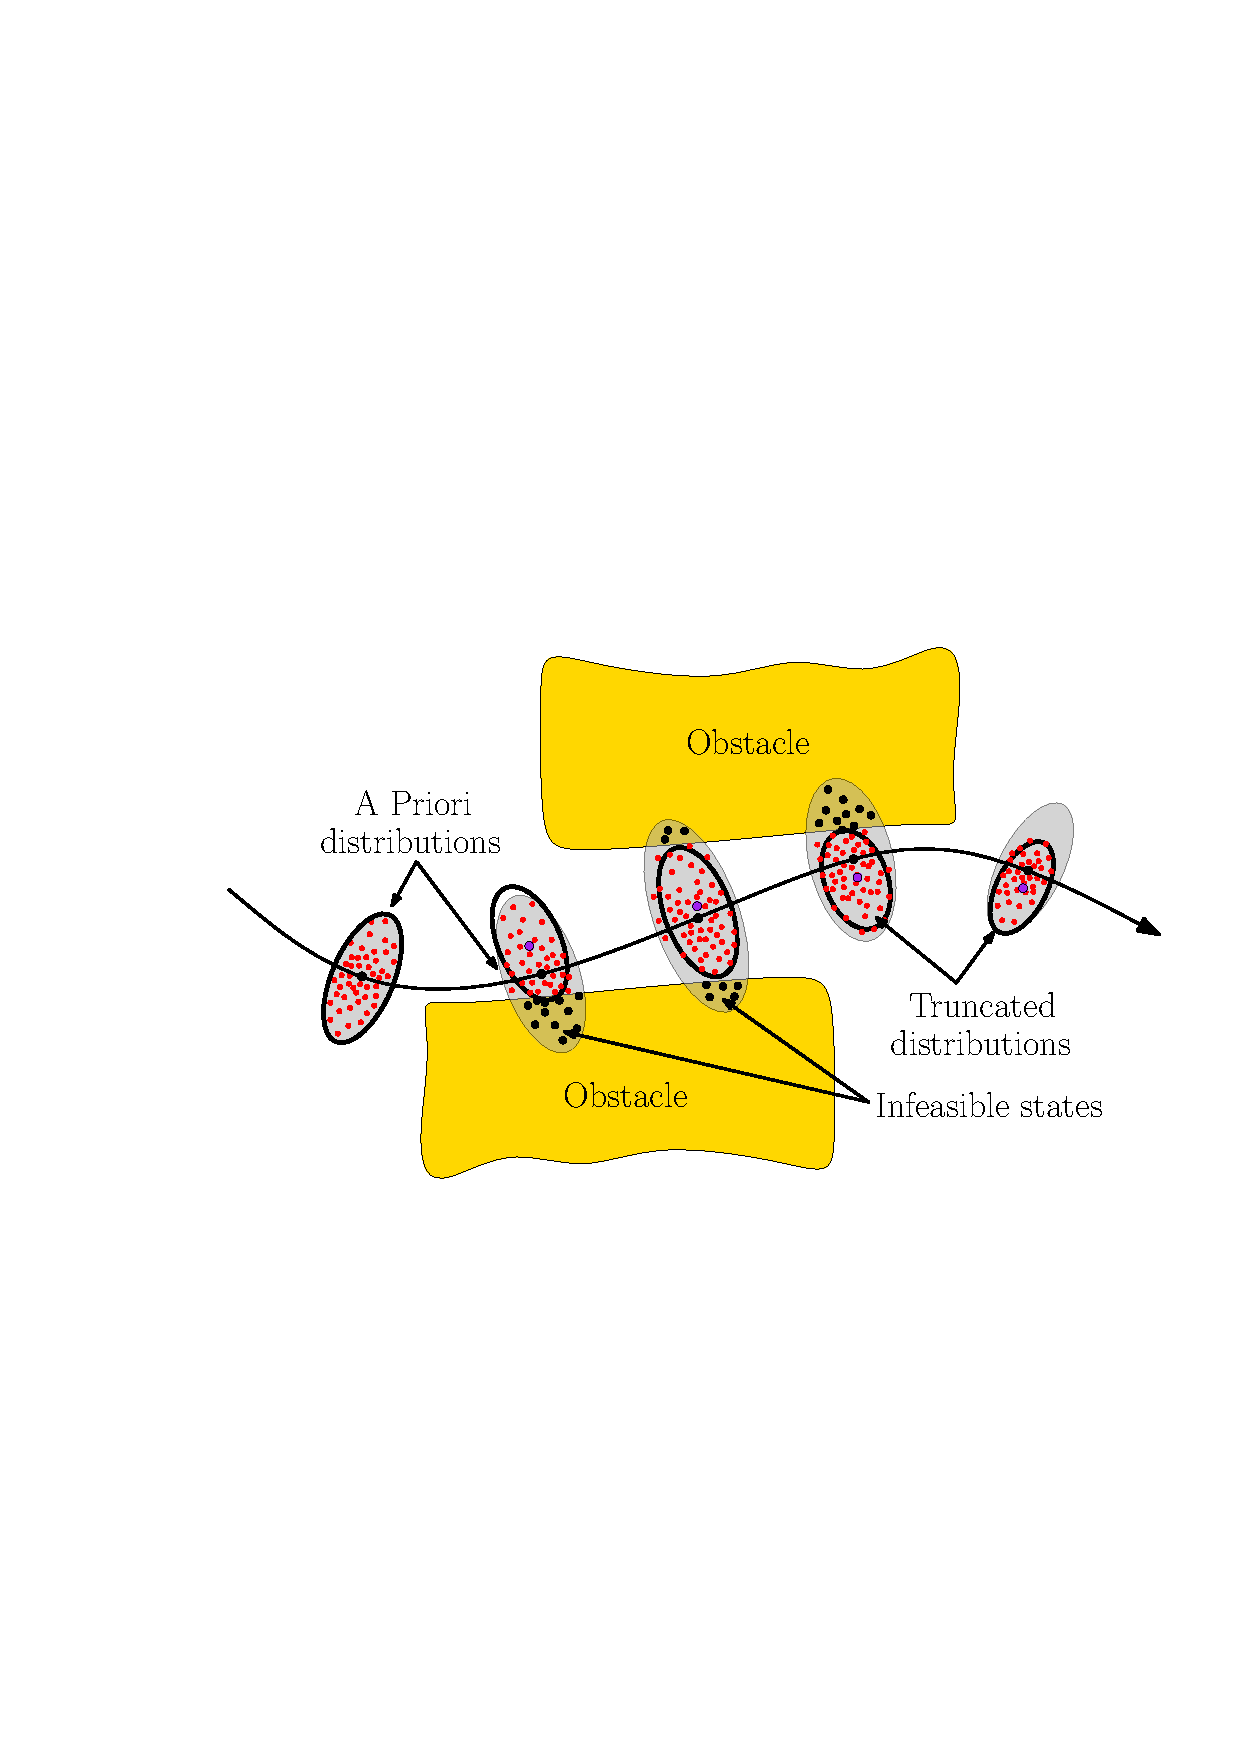
\includegraphics[width=225pt,clip]{figures/truncatedGaussians3.pdf}
\vspace{-5pt}
\caption{We estimate the probability of collision for a motion plan based on \emph{a priori} probability distributions of the robot state. The probability of collision at each stage of the plan is conditioned on the previous stages being collision free. We compute truncated \emph{a priori} distributions that discount plan executions (black dots) that collide with obstacles. Propagating the truncated distributions (black ellipses) accounts for only the collision free samples (red dots), resulting in accurate estimation of the probability of collision. Prior methods that use the unconditional distributions (gray ellipses) to estimate the collision probability result in an overly conservative estimate.}
\label{fig:teaser}
\vspace*{-15pt}
\end{figure}

Prior work on motion planning under uncertainty has used both sampling-based and analytical approaches to estimating probability of collision. Na\"{i}ve Monte Carlo sampling strategies can estimate the probability of collision by computing the ratio of the number of simulated executions that are collision free. This approach requires a large number of simulations to obtain a reliable estimate, which requires more computation time than analytical approaches. Monte Carlo sampling also offers no guarantee that it will not underestimate the probability of collision, resulting in violation of safety requirements.
Under the assumption of Gaussian motion and sensing uncertainty, probability of collision can be estimated quickly based on \emph{a priori} probability distributions of the robot state \cite{vandenBerg11_IJRR, Bry11_ICRA, Vitus11_ICRA}. However, prior methods typically ``approximate'' the collision probability of a plan by assuming the probabilities of collision at stages along the plan are independent. Formally speaking, let $\mathbf{x}_t \in \mathcal{X}$ denote the state of the robot at stage $t$ along the plan, and $\mathcal{X}_{F} \subset \mathcal{X}$ denote the feasible space not occupied by obstacles. Prior methods assume that the probability that a plan consisting of $\ell$ stages is collision free is given by $p(\bigwedge_{t = 0}^{\ell} \; \mathbf{x}_t \in \mathcal{X}_{F}) \approx \prod_{t = 0}^\ell p(\mathbf{x}_{t} \in \mathcal{X}_{F})$. This yields an overly conservative estimate of the probability of collision (see Fig.\ \ref{fig:teaser}), which might result in overly conservative motion plans and, depending on the safety required by the motion planner, may result in failure to find a feasible plan even if one exists.

We propose an analytic approach to estimating the probability of collision that accounts for the fact that the distribution of the state at each stage along the plan is \emph{conditioned} on the previous stages being collision free, i.e., the probability that a plan is collision free is given by $p(\bigwedge_{t = 0}^{\ell}\; \mathbf{x}_t \in \mathcal{X}_{F}) = \prod_{t = 0}^\ell p(\mathbf{x}_{t} \in \mathcal{X}_{F}\; |\; \bigwedge_{i = 0}^{t-1} \; \mathbf{x}_i \in \mathcal{X}_{F})$. This amounts to propagating the \emph{a priori} distributions forward in time in such a way that instances that collide with obstacles are discounted from the propagation (Fig.\ \ref{fig:teaser}). For this we propose a novel method to truncate the \emph{a priori} distributions with respect to obstacles, approximate the truncated distributions by Gaussians, and propagate the truncated distributions forward in time. This results in an accurate estimate of the conditional distributions, and consequently, enables accurate estimation of the collision probability.

%Even though the exposition outlines a method to truncate the distributions with respect to obstacles, we can directly apply this methodology to estimate the \emph{a priori} distributions with other constraints on the state variables (such as imposing limits on velocity, acceleration etc. of the robot).
Our method can be used to quantify the safety of a plan \cite{vandenBerg11_IJRR, Patil11_RSS}, to improve quality of estimation of collision chance constraints \cite{Bry11_ICRA, Vitus11_ICRA}, or to elegantly account for hard state constraints imposed by obstacles in optimization based \cite{Erez10_UAI} or inference based \cite{Toussaint09_ICML} planning methods. Our truncation approach is also directly applicable to the important problem of optimal state estimation with hard state constraints \cite{Book:Simon06}.

We present simulation-based results for two scenarios with with stochastic dynamics and partial, noisy state feedback: (1) a car-like robot with second-order dynamics, and (2) a nonholonomic bevel-tip flexible needle. Our method was orders of magnitude faster than na\"{i}ve sampling based methods and computed a significantly more accurate estimate of collision probability compared to prior analytical methods.
